\documentclass{ecnreport}

\stud{Master 1 CORO / Option Robotique}
\topic{Robot Operating System}
\author{O. Kermorgant}

\begin{document}

\inserttitle{Robot Operating System}

\insertsubtitle{Lab 4: the navigation stack}

\section{Goals}

This lab aims to discover the capabilities of the \link{https://navigation.ros.org/}{ROS 2 navigation stack}. This set of packages are designed to have one or several mobile robots move in a known environment. Robots are assumed to carry laser scanners\footnote{other exteroceptive sensors (camera, depth-camera, ultrasonic) may be used but most tutorial assume laser scanners}, that give a local sensing of their surroundings. 
These laser scans are used:
\begin{itemize}
 \item To build the map, if the environment is not known yet (SLAM, Simultaneous Localization And Mapping)
 \item To localize on a known map (pure localization)
 \item To detect and avoid obstacles that are not on the map (obstacle avoidance)
 \end{itemize}
 
\subsection{The navigation2 packages}
 
By using the navigation stack you will get familiar with:
\begin{itemize}
 \item Standard 3D frames for mobile platforms (\link{https://www.ros.org/reps/rep-0105.html}{REP 105})
 \item Capabilities of the navigation2 stack:
 \begin{itemize}
  \item SLAM
  \item Map server: take a map and publish it to other nodes
  \item Localization: estimate the pose of the robot by comparing laser readings to the map
  \item Planning: compute the path to a given goal position on the map
  \item Control: track the path, avoid unexpected obstacles if needed
 \end{itemize}
\end{itemize}

In this lab, SLAM is not performed as it takes too much time. Indeed, taking 15 or 20 min of raw laser data and create a map out of it is quite computationally intensive. Some online tutorial explain how to do it from a bag file, either in ROS 1 or ROS 2.

Here we thus assume that a map is given.

\subsection{Maps in ROS}

In ROS 1 or 2, a map is a combination of two files:\\

\begin{minipage}{.6\linewidth}
 \begin{itemize}
  \item An image file describing occupied (black) / free (white) or unknown (grey) occupancy grid
  \item A YAML file describing the link between image space (in pixels) and Euclidean space (in meter)
  \begin{pythoncodelarge}
# map image
image: batS.pgm  
# size of one pixel in meters
resolution: 0.020000
#coordinates of the pixel (0,0)
origin: [-6.064576, -10.118860, 0.000000]
negate: 0
occupied_thresh: 0.65 
free_thresh: 0.196
  \end{pythoncodelarge}
 \end{itemize} 
\end{minipage}
\begin{minipage}{.05\linewidth}
 ~
\end{minipage}
\begin{minipage}{.33\linewidth}
 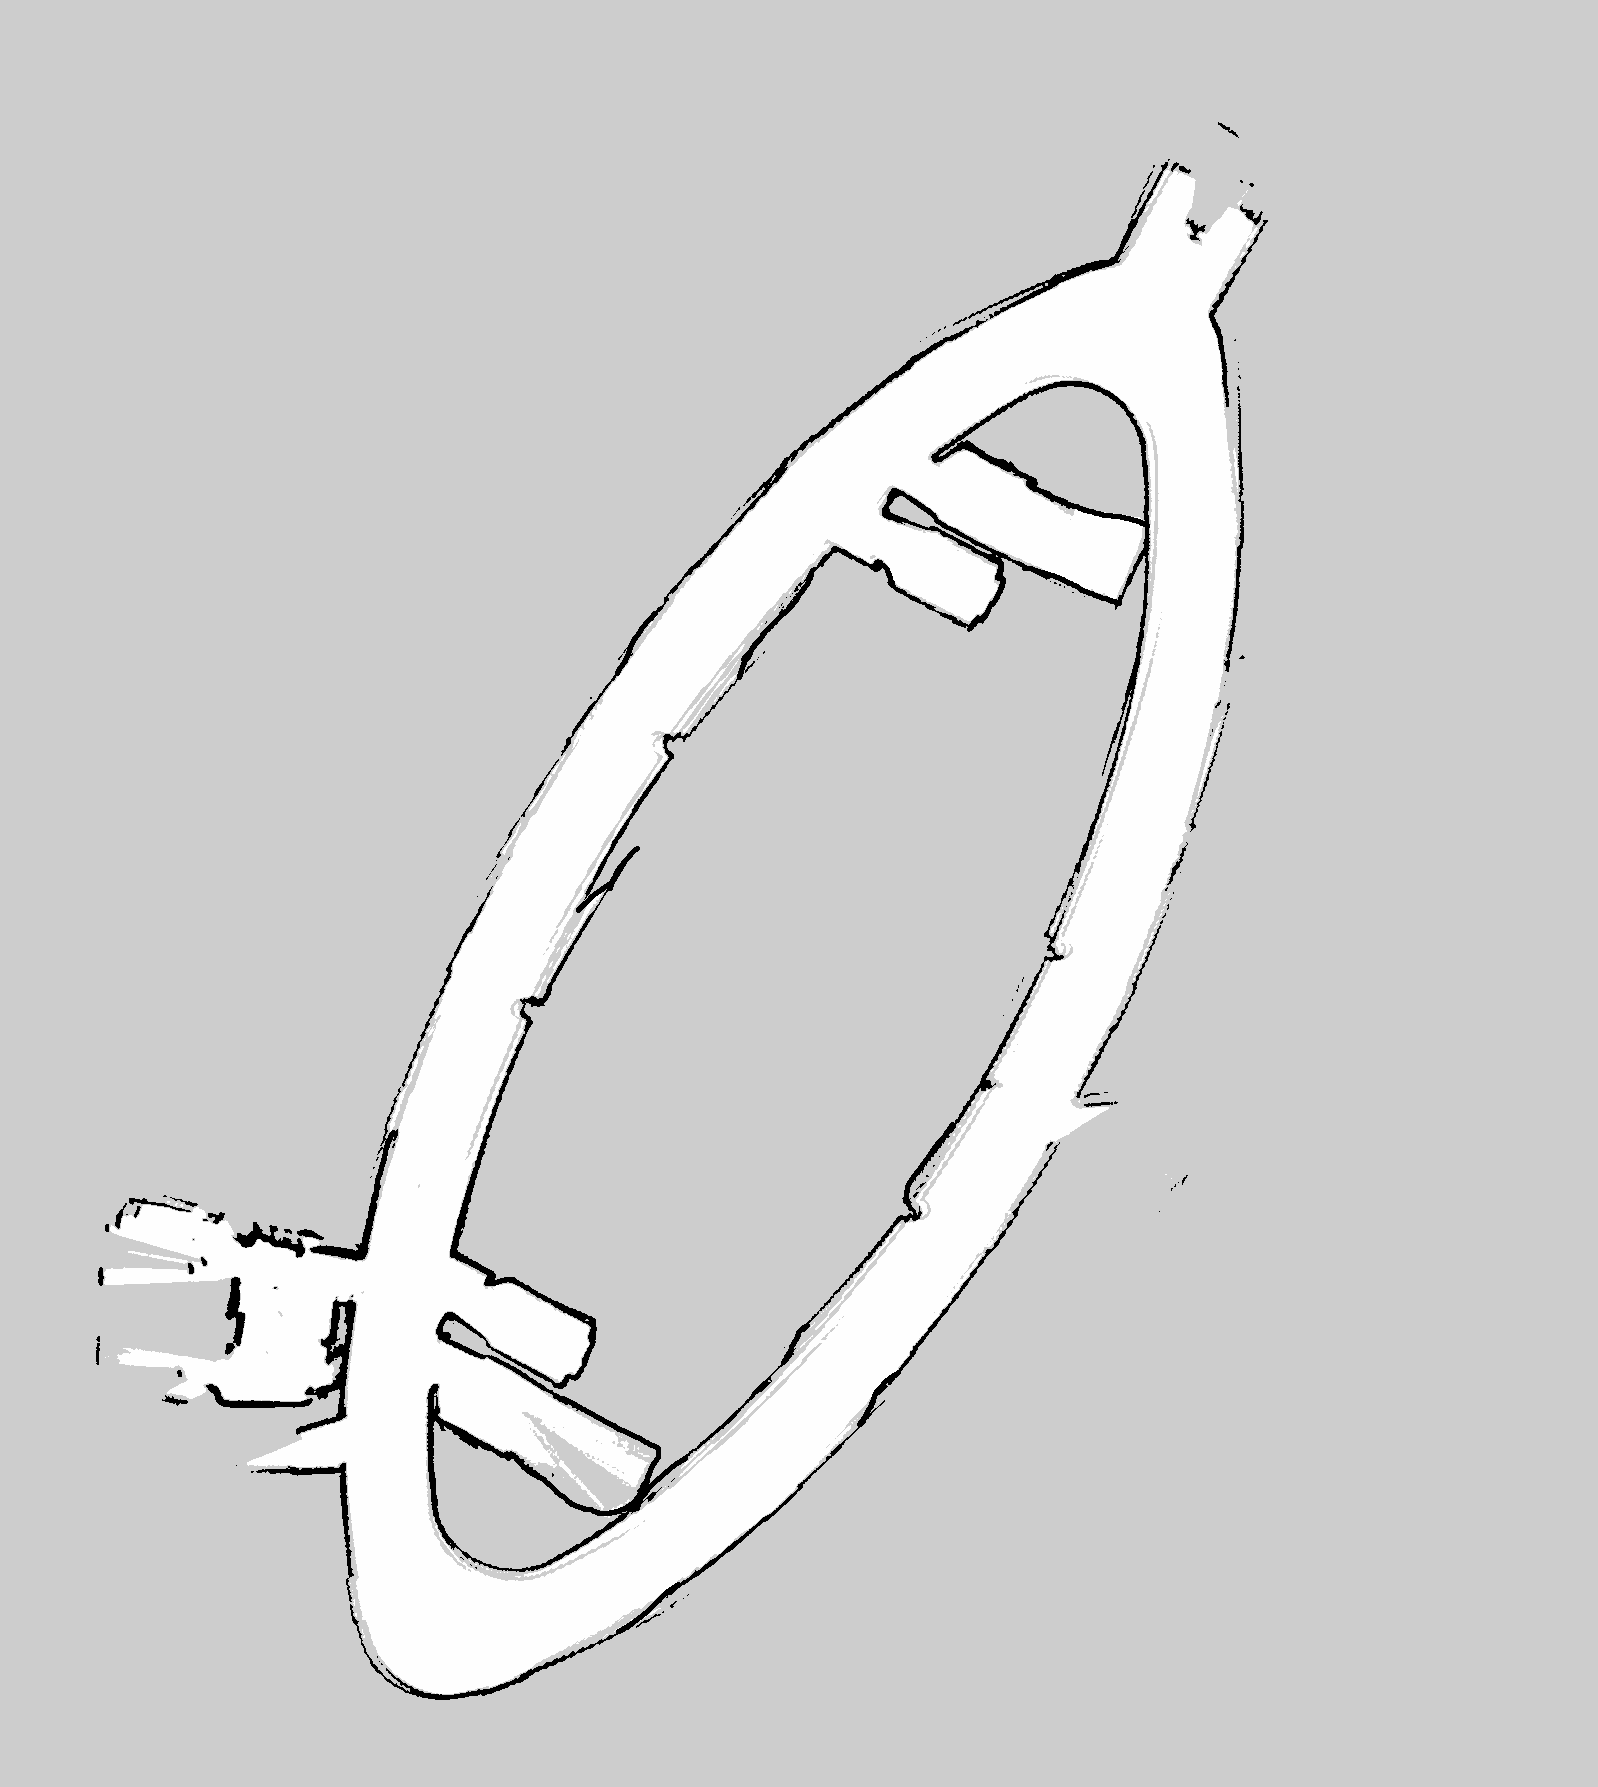
\includegraphics[width=\linewidth]{batS}
\end{minipage}~\\

Such maps can be generated from a SLAM algorithm, and are the core data of any localization or navigation capabilities.

Here, the map was built by running a Turtlebot robot on the 4th floor of Building S on the Centrale Nantes campus. The room on the bottom-left is actually my office.


\subsection{Compiling and running the simulation}

The package should be compiled by \texttt{colcon} to have the files discoverable by ROS 2:
\begin{bashcodelarge}
 ros2ws
 cd ~/ros2
 colbuild --packages-select lab4_navigation
\end{bashcodelarge}

In this lab, the map is also used as a simulated environment. Simulated robots can move and measure their distance to the walls or other robots through a laser scanner. The environment is run with:
\begin{bashcodelarge}
 ros2 launch lab4_navigation simulation_launch.py 
\end{bashcodelarge}This will create two windows:
\begin{itemize}
 \item \texttt{Simulator 2D} which is the actual simulation (without any robot for now)
 \item \texttt{Rviz2} which is the main visualization GUI in ROS.
\end{itemize}
The windows can be kept alive during the whole lab.

\newpage

\section{Pure localization}

In the first step, pure localization will be considered with manual control. This can be done for one robot by running:
\begin{bashcodelarge}
 ros2 launch lab4_navigation bb8_amcl_launch.py
\end{bashcodelarge}
The BB8 robot is displayed in the simulation (true pose) and in RViz (estimated pose).\\

For this initial run, things should not go as planned. Identify which topics AMCL subscribes to, versus which topics should be used instead. These topics (and frames of interest) are defined in the file \texttt{urdf/amcl\_param.yaml} that sets a number of ROS parameters for AMCL. \\Change their names either here, or using remappings in \texttt{bb8\_amcl\_launch.py}. 

\subsection{AMCL}

The set of all red arrows represents how AMCL (Adaptative Monte-Carlo Localization) works. Here localization is not done eg with a Kalman Filter but with a particle filter. Each particle is a state candidate (pose + velocity). The overall estimation is the center of gravity of all particles.

From laser readings, some particles are pruned as they are not consistent with the scans.

\subsection{Interaction with RViz}

You can reset the estimation by using the \texttt{2D Pose Estimate} button in RViz. Try giving a completely wrong estimate and check that:
\begin{itemize}
 \item The simulated robot is still at the same place in the simulation window
 \item Its pose is not the same in RViz, and the laser scans are not aligned with the walls
\end{itemize}

\subsection{Moving the robot}

This launch file also runs a slider publisher to move BB8 as a 2-0 robot with a $(v,\omega)$ command.\\
When the robot has a slight estimation error, try to have it rotate (pure $\omega$ command) to check if AMCL is able to realign the laser scans to the walls. \\
On the opposite, try to put the robot at a similar but different place (the floor being almost symmetric).
AMCL will not be able to tell that the robot position is completely wrong, as the laser scans can be correctly aligned with the known walls.

\subsection{Nodes and frames}

Use \texttt{rqt\_graph} and TF tools (\texttt{tf2\_tools view\_frames.py}) to display the nodes and the frames:
\begin{itemize}
 \item Which frames are linked to the robot, to the map, in-between?
 \item Which node publishes each frame transform?
 \item Especially, what do the following transforms correspond to and which nodes are responsible for them:
 \texttt{map} $\rightarrow$ \texttt{bb8/odom} $\rightarrow$ \texttt{bb8/base\_link}.
\end{itemize}

\section{Planning and control}

In this part, we will consider a perfect localization. Instead of running AMCL (that can be CPU intensive), a perfect estimation 
will be published by running the \texttt{vel2joints} node with the parameter \texttt{static\_tf} set to True.

Many nodes have to be run to have full capabilities of the navigation stack, as shown in the following figure:
\begin{center}
 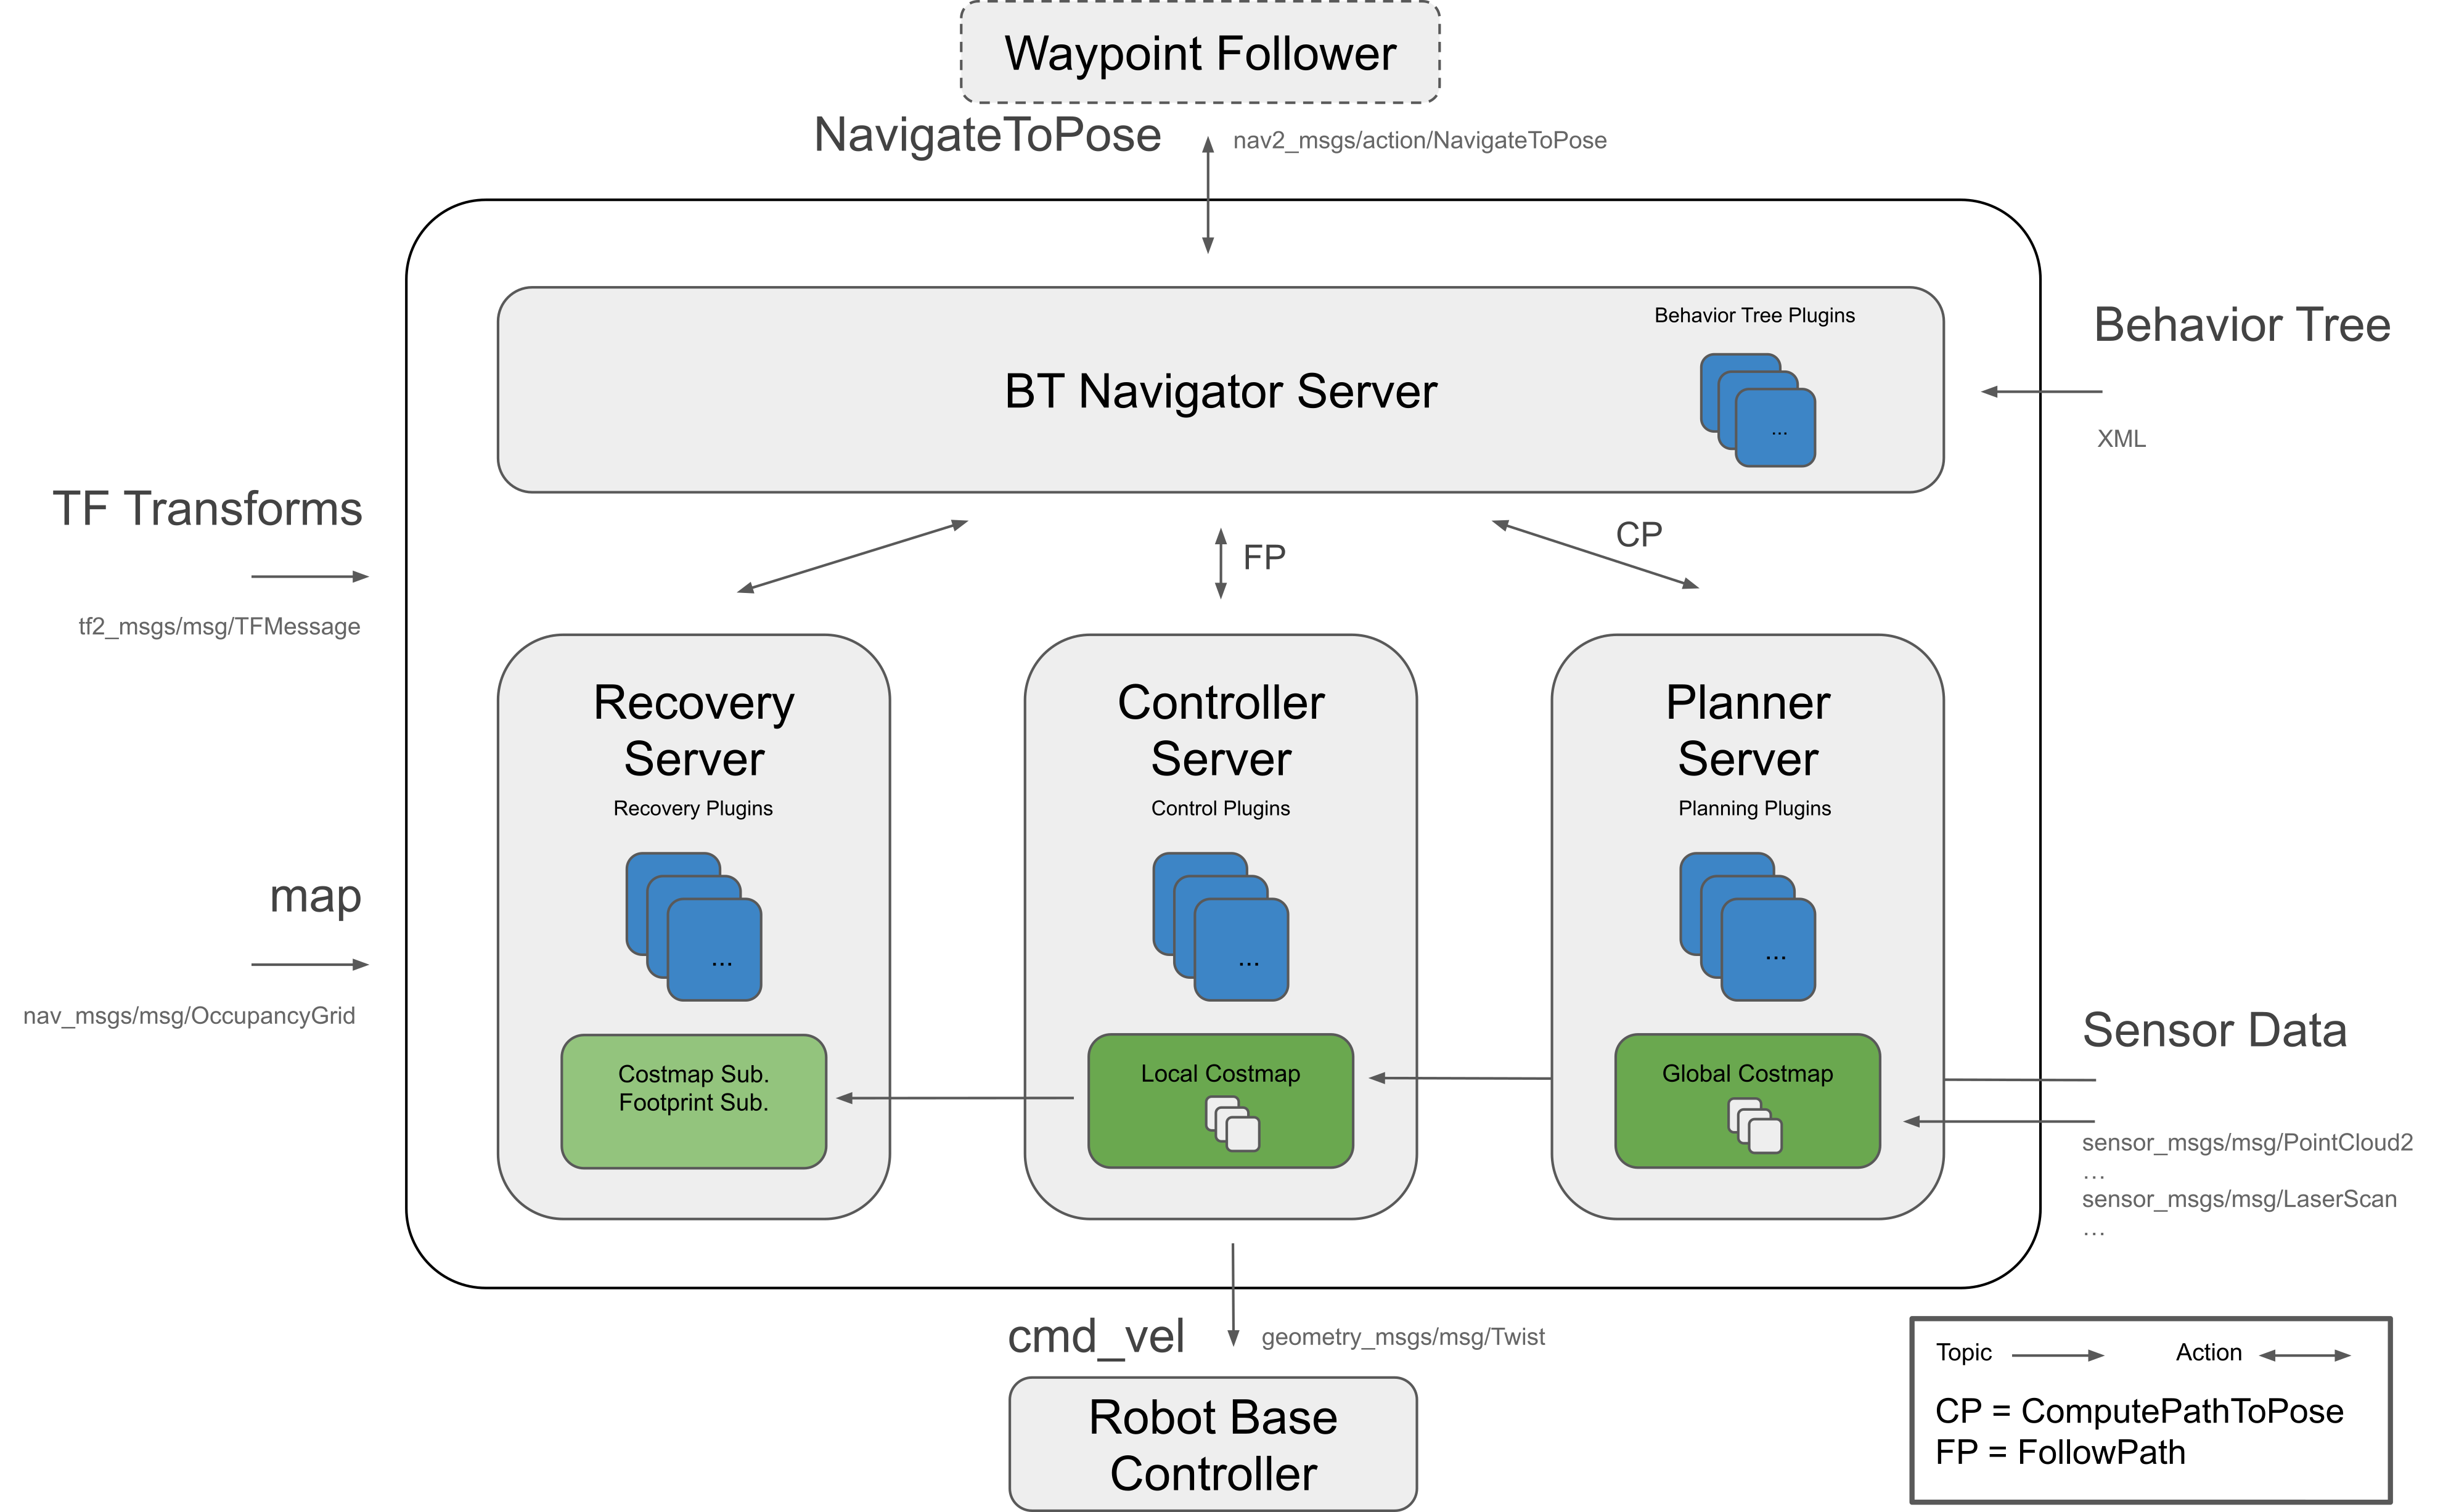
\includegraphics[width=.7\linewidth]{nav2_architectural_diagram}
\end{center}

\subsection{Creating a robot-generic navigation launch file}

Four robots are defined in the lab package. There are two BB-type (BB8 / BB9) and two D-type (D0 / D9).\\

Copy/paste the \texttt{bb8\_amcl\_launch.py} file to a new \texttt{spawn\_launch.py} file. Then, update this file such that:
\begin{itemize}
 \item It takes a new argument called \texttt{'robot'} with default value \texttt{'bb8'}.
 \item It runs the \texttt{vel2joints} node with a parameter \texttt{static\_tf} set to True. 
\end{itemize}

Install this file by compiling the package again (it is the last time!).\\

The type of a robot can be deduced at run-time with the following lines in the launch file:
\begin{pythoncodelarge}
robot = sl.arg('robot')
robot_type = sl.py_eval("''.join(c for c in '", robot, "' if c.isalpha())") 
\end{pythoncodelarge}\texttt{robot\_type} will be either \texttt{'bb'} or \texttt{'d'}. In practice, it runs a bit of Python code to extract the non-digital characters of the robot name: \texttt{'bb8'} thus becomes \texttt{'bb'}, and so on.\\

The corresponding model can be loaded accordingly:
\begin{pythoncodelarge}
sl.robot_state_publisher('lab4_navigation', 
                          sl.name_join(robot_type, '.xacro'),
                         'urdf', xacro_args={'name': robot})
\end{pythoncodelarge}this line will read either \texttt{bb.xacro} or \texttt{d.xacro} depending on the passed \texttt{robot} argument. 

\subsection{Allowing for manual control}

Create a new argument called e.g. \texttt{use\_nav} with default value False. \\

A first conditionnal block is to run the slider publisher only if this parameter is indeed False. This is done with the following syntax:
\begin{pythoncodelarge}
with sl.group(unless_arg='use_nav'):
    cmd_file = sl.find('lab4_navigation', 'cmd_sliders.yaml')
    sl.node('slider_publisher', 'slider_publisher', arguments=[cmd_file])
\end{pythoncodelarge}

Test that the launch file works properly and that you can run BB8 in a terminal, and another robot in another terminal. You should have two slider publishers, one for each robot. In RViz, BB8 and D0 are already setup but you can easily add description / laser scanner display for the other robots.

\subsection{Running navigation nodes}

If the parameter \texttt{use\_nav} is True, then the slider publisher should be replaced by the navigation nodes. This is done by creating a block under the condition:
\begin{pythoncodelarge}
with sl.group(if_arg='use_nav'):
    # many things to do in this case
\end{pythoncodelarge}

In \texttt{bb8\_amcl\_launch.py}, the AMCL node in run through a life cycle manager. This should be the case for all navigation nodes. This can be done through a loop in the launch file, where each navigation node is identified by its package and its executable:
\begin{pythoncodelarge}
nav_nodes = [('nav2_controller','controller_server'), 
        ('nav2_planner','planner_server'),
        ('nav2_bt_navigator','bt_navigator'),
        ]
for pkg,executable in nav_nodes:
    # run this executable from this package
    # add the executable name to some list of nodes to be managed by life cycle manager
\end{pythoncodelarge}Analyze the syntax used to run a node and add it to the life cycle manager, and run all the navigation nodes.\\

The parameter file that should be used is now \texttt{nav\_param.yaml} instead of \texttt{amcl\_param.yaml}. At this time, you can run:
\begin{bashcodelarge}
# runs BB8 with nav capabilities
ros2 launch lab4_navigation spawn_launch.py use_nav:=True
# runs D0 with manual control (in another terminal)
ros2 launch lab4_navigation spawn_launch.py robot:=d0
 \end{bashcodelarge}
 Nothing will work as planned with the navigation however. Indeed, the nodes are not correctly configured.

\subsection{Adapting the parameters}

Compare the files \texttt{amcl\_param.yaml} and \texttt{nav\_param.yaml}. The first one explicitely writes that the node is run in the \texttt{bb8} namespace. Also, the frames of interest (\texttt{bb8/odom}, \texttt{bb8/base\_link}) are explicitely given in the parameter file.\\

It is not the case for \texttt{nav\_param.yaml}. And it should not, as this file may be used for various robots that all have their own namespace and frame prefix.\\
We will use a launch capability to update the parameters during launch. Do to that, import the following function in the launch file:
\begin{pythoncodelarge}
from nav2_common.launch import RewrittenYaml
\end{pythoncodelarge}

This function takes the following arguments:
\begin{itemize}
\item \texttt{source\_file}: the initial parameter file
\item \texttt{root\_key}: any namespace to be used (in our case: the robot variable)
\item \texttt{param\_rewrites}: a dictionary of parameters names with their new value. Such required changes are defined below.
\item \texttt{convert\_types}: should be set to True
\end{itemize}

Then, the output of the function should be passed instead of the actual parameter file:
\begin{pythoncodelarge}
configured_params = RewrittenYaml(source_file = ...,
                                    root_key = ..., 
                                    param_rewrites = ...,
                                    convert_types = True)
sl.node(..., parameters = [configured_params])
\end{pythoncodelarge}

Parameters that need to be rewritten are:
\begin{itemize}
 \item All frames, such as \texttt{odom} or \texttt{base\_link}, that should be prefixed with the robot name to make them look like \texttt{bb8/odom} or \texttt{d0/base\_link}. Note that the name of the parameter is to be used in \texttt{param\_rewrites}, not its default value. For example, \texttt{base\_link} usually appears as the \texttt{robot\_base\_frame} parameter in \texttt{nav\_param.yaml}.
 \item The robot radius, that has default value 0.105 and is used for obstacle avoidance. This should be set to '.27' for a BB-type or '.16' for a D-type. This can be done dynamically:
\begin{pythoncodelarge}
# robot radius depends on the robot type
robot_rad = sl.py_eval("'", robot_type, "'=='bb' and .27 or .16")
\end{pythoncodelarge}
\item The Behavior Tree file, that is usually found in the \texttt{nav2\_bt\_navigator} package. Use this syntax to pass it to the rewritten params:
\begin{pythoncode}
 'default_bt_xml_filename': sl.find('nav2_bt_navigator','navigate_w_replanning_time.xml')   # or another file
\end{pythoncode}
\end{itemize}

\subsection{Playing with navigation}

Once the launch file is updated, you can spawn BB8 with nav capabilities, and another one with manual control. The \texttt{2D Goal Pose} button in RViz allows giving a pose setpoint for BB8 to reach. A trajectory will be found (hopefully) and the control with begin.\\

Try to have the manually-controlled robot annoy BB8 by going on the planned path. It should be detected by the laser scanner, and BB8 should be able to modify its trajectory.\\

You can also inspect the \texttt{nav\_param.yaml} file and try tuning the control / planning parameters. For instance, it may be allowed or not to move backwards, and various thresholds are defined to consider that the desired pose is reached.


\section{Conclusion}

In this lab, the navigation stack is detailed. You have seen that a single, potentially well-tuned, configuration file can be used for several robots by updating it on-the-fly during launch. The only frame common to all robots is the map, while any other frame is either published by the localization node (odom) or by the robot state publisher. \\

Many behaviors can be defined to tune how a robot navigates. Feel free to try various Behavior Tree files and see the impact on the robot.

\end{document}
